\subsubsubsection{reducing}

\hspace*{\fill}

\indent ReducingGate is used for computes $\text{output} = \text{old\_acc} + \sum C_i \cdot\alpha^i$ in the base field.

The trace structure for this gate is like this:

\begin{figure}[!ht]
    \centering
    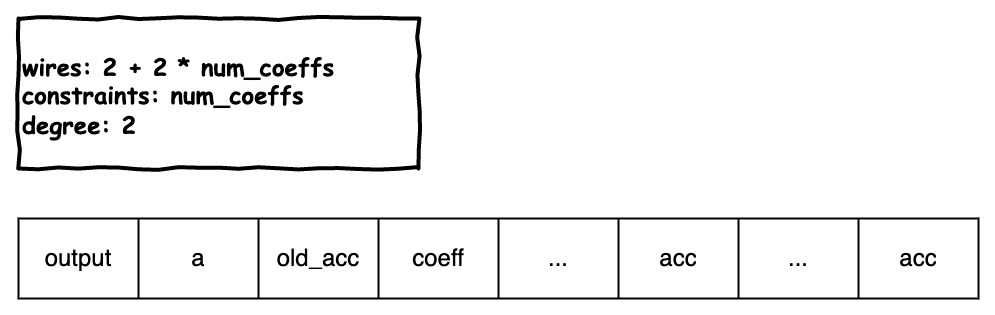
\includegraphics[width=0.6\textwidth]{gates/reducing.jpeg}
    \caption{ReducingGate}
    \label{fig:reducing}
\end{figure}

The constraint flow is relatively intuitive, initializing acc to old\_acc, then cumulative computation of polynomials by coeff in turn, 
and constraining the intermediate results of each step with acc.

\begin{lstlisting}[language=rust]
for i in 0..self.num_coeffs {
    let coeff = builder.convert_to_ext_algebra(coeffs[i]);
    let mut tmp = builder.mul_add_ext_algebra(acc, alpha, coeff);
    tmp = builder.sub_ext_algebra(tmp, accs[i]);
    constraints.push(tmp);
    acc = accs[i];
}
\end{lstlisting}

The number of constraints is equal to the number of coefficients. The polynomial degree is 2 which happens when calculating $\text{coeff}_i * \alpha$, sum up does not increase degree.

ReducingExtensionGate is like ReducingGate, just computations happen in the extension field, and constrain logic is all the same.
